\documentclass[11pt,a4paper]{book}
\usepackage{xltxtra}
\usepackage{fontspec} %指定新罗马字体
\usepackage{float}
\usepackage{listings} % 代码
\usepackage{xeCJK}  %指定中文字体
\usepackage[top=0.8in,bottom=0.8in,left=1.2in,right=0.6in]{geometry}
\usepackage[bookmarksnumbered,colorlinks,linkcolor=black,anchorcolor=black,citecolor=black]{hyperref}
\usepackage{epigraph}
\usepackage{amsmath}
\usepackage{underscore} 
\usepackage{indentfirst}
\setlength{\parindent}{2em}
\lstset{ 
	frame=shadowbox,
	numbers=left,
	numberstyle=\tiny,
	language=python,
	stepnumber=1,
	commentstyle=\small,
	extendedchars=false,
	escapeinside=`` ,
	showstringspaces=false,
	columns=fullflexible,
	breaklines=true,                 % automatic line breaking only at whitespace
	breakautoindent=true,%
        breakindent=4em, %
	captionpos=b,                    % sets the caption-position to bottom
	tabsize=4,
%	basicstyle=\ttm,
}
\setmainfont{Times New Roman}
\setsansfont{Helvetica}
\setmonofont{Courier}
\setCJKmainfont[BoldFont={STXihei},ItalicFont={STKaiti}]{STSong}
%\setCJKsansfont[BoldFont=STXihei]{STKaiti}
%\setCJKmonofont{STSong}

\title{linux从入门到放弃}
\author{蔚雷}
\date{\today}

\usepackage{filecontents}
\usepackage{biblatex}

%\begin{filecontents}{mybib.bib}
%@unpublished{Survey2014,
%  title={Survey on the access to finance of enterprises},
%  author={Sophie Doove and Petra Gibcus and Ton Kwaak and Lia Smit and Tommy Span},
%  year=2014,
%  note ={Accessed 16 June 2017. http://wwwe.ansa.it/documents/1415814222451\_Rapporto.pdf/ },
%}
%	@unpublished{
%		tile={}
%		}
%% 在document使用链接
%% \citet{Survey2014}
%% \printbibliography
%\end{filecontents}
%\bibliography{mybib} 

%\bibliographystyle{unsrt}
%\bibliography{sample}


\begin{document}

\maketitle

\tableofcontents 

\mainmatter

\chapter*{Preface}

运维工作四五年,所做之事已无乐趣,了无生趣,总结运维之事,安装系统,部署服务,改参数,调配置,部署代码,
使用工具大致都相仿,什么shell,kickstart,cobbler,ansible,salt,nginx,apache,php,tomcat,keepalived,mysql,git,svn
jenkins.等之类软件,用什么都不能说精,也不能说不会,昏昏沉沉一年过去,不闻其道,不见其神,只会其术,
可谓一塌糊涂,这样下去无非是浪费时间,不如借此时机,把所学之事整理成成文,

\chapter{自动化安装系统}


Redhat系主要有两种方式安装系统Kickstart和Cobbler。
Kickstart是一种无人值守的安装方式。它的工作原理是在安装过程中记录人工干预填写的各种参数,并生成一个名为ks.cfg的文件。如果在自动安装过程中出现要填写参数的情况,安装程序首先会去查找ks.cfg文件,如果找到合适的参数,就采用所找到的参数;如果没有找到合适的参数,便会弹出对话框让安装者手工填写。所以,如果ks.cfg文件涵盖了安装过程中所有需要填写的参数,那么安装者完全可以只告诉安装程序从何处下载ks.cfg文件,然后就去忙自己的事情。等安装完毕,安装程序会根据ks.cfg中的设置重启/关闭系统,并结束安装。

Cobbler集中和简化了通过网络安装操作系统需要使用到的DHCP、TFTP和DNS服务的配置。Cobbler不仅有一个命令行界面,还提供了一个Web界面,大大降低了使用者的入门水平。Cobbler内置了一个轻量级配置管理系统,但它也支持和其它配置管理系统集成,如Puppet,暂时不支持SaltStack。

在这之前需要了解几个概念,PXE(pre-boot execution environment) 预启动执行环境,通过网络接口启动计算机,不依赖本地存储设备或本地已安装的操作系统,它的工作模式是client/server工作模式,PXE客户端会调用网际协议IP,用户数据报协议(UDP),动态主机设定(DHCP),小型文件传输协议(TFTP)等网络协议。
PXE工作过程

DHCP(Dynamic Host Configuration Protocol,动态主机配置协议)通常被应用在大型的局域网络环境中,主要作用是集中的管理、分配IP地址,使网络环境中的主机动态的获得IP地址、网关地址、DNS服务器地址等信息,并能够提升地址的使用率。端口号67,安装系统时开启,安装后关闭

 TFTP(Trivial File Transfer Protocol,简单文件传输协议)是TCP/IP协议族中的一个用来在客户机与服务器之间进行简单文件传输的协议,提供不复杂、开销不大的文件传输服务。端口号为69。

\ref{Fig:pxe-step}

\begin{enumerate}
\item PXE客户端(需要安装系统的机子) 通过PXE BOOTROM(自启动芯片)会以UDP发送一个广播,向本网络中的DHCP服务器索取IP
\item DHCP服务端收到客户端的请求,验证是否来至合法的PXE clinet的请求,验证通过它将给客户端一个响应其中包含为客户端分配的IP地址,PXELINUX启动程序(TFTP)位置以及配置文件所在位置
\item 客户端收到服务端的回应后会再请求传送启动所需文件:pxelinux.0, pxelinux.cfg/default. vmlinuz, initrd.img
\item 服务端通过TFTP通讯协议从Boot server下载启动安装程序所必需的文件,然后根据该文件中定义的引导顺序,启动linux安装程序的引导内核
\item 客户端通过pxelinux.cfg/default文件成功引导linux安装内核后,安装程序必须确定通过什么安装介质来安装linux,如果通过网络安培(nfs,ftp,http,),便会初始化网络,并定位安装源位置。此时会读取default文件中指定的自动应答文件ks.cfg所在位置,根据该位置请求下载该文件
\item 从服务端下载完ks.cfg文件后,通过该文件找到os server,并按照文件的配置请求下载安装过程需要的软件包。os server 和客户端建立连接后,将开始传输软件包,客户端将开始安装操作系统。安装完成后将重新引导计算机。
\end{enumerate}

这里有个问题,在第2步和第5步初始化2次网络了,这是由于PXE获取的是安装用的内核以及安装程序等,而安装程序要获取的是安装系统所需的二进制包以及配置文件。因此PXE模块和安装程序是相对独立的,PXE的网络配置并不能传递给安装程序,从而进行两次获取IP地址过程,但IP地址在DHCP的租期内是一样的。

\section{kickstart 安装部署步骤}
服务端环境环境:CentOS release 6.7 (Final)  ip 10.0.0.151 ,selinux,防火墙关闭, 首先安装DHCP,TFTP, HTTP服务

\lstinputlisting{./cobble/codes/installDhcp.sh}

好吧让我们来看看效果如果出现下面画面证明配置成功啦

\ref{Fig:kickstartDhcp}

配置支持PXE的启动程序 syslinux
syslinux是一个功能强大的引导加载程序,而且兼容各种介质。SYSLINUX是一个小型的Linux操作系统,它的目的是简化首次安装Linux的时间,并建立修护或其它特殊用途的启动盘。如果没有找到pxelinux.0这个文件,可以安装一下。

\lstinputlisting{./cobble/codes/installSyslinux.sh}

\subsection{创建ks.cfg文件}
kickstart是为了避免安装操作系统的过程中的交互操作,只要定义好一个kickstar自动应答配置文件ks.cfg,并让安装程序知道该配置文件的位置,就可以在安装中读取配置文件来安装系统。

生成kickstaart配置文件的三种方法:

每安装好一台Centos机器,Centos安装程序都会创建一个kickstart配置文件,记录你的真实安装配置。如果你希望实现和某系统类似的安装,可以基于该系统的kickstart配置文件来生成你自己的kickstart配置文件。(生成的文件名字叫anaconda-ks.cfg位于/root/anaconda-ks.cfg)

Centos提供了一个图形化的kickstart配置工具。在任何一个安装好的Linux系统上运行该工具,就可以很容易地创建你自己的kickstart配置文件。kickstart配置工具命令为redhat-config-kickstart(RHEL3)或system-config-kickstart(RHEL4,RHEL5).网上有很多用CentOS桌面版生成ks文件的文章,如果有现成的系统就没什么可说。但没有现成的,也没有必要去用桌面版,命令行也很简单。

阅读kickstart配置文件的手册。用任何一个文本编辑器都可以创建你自己的kickstart配置文件。

ks.cfg 文件组成大致分为3段

命令段:键盘类型,语言,安装方式等系统的配置,有必选项和可选项,如果缺少某项必选项,安装时会中断并提示用户选择此项的选项

* 软件包段

语法基本可以写成

\begin{lstlisting}
%packages
@groupname:指定安装的包组
package_name:指定安装的包
-package_name:指定不安装的包
* 脚本段(可选)

%pre:安装系统前执行的命令或脚本(由于只依赖于启动镜像,支持的命令很少)
%post:安装系统后执行的命令或脚本(基本支持所有命令)
\end{lstlisting}

首先要使用grub-crypt生成一个密码用于root密码,编写ks配置文件放到/var/www/html/ks_config/CentOS-6.7-ks.cfg,

%\lstinputlisting{./codes/cobble/CentOS-6.7-ks.cfg}

优化脚本,也需要放在下面。/var/www/html/ks_config/optimization.sh

%\lstinputlisting{./codes/cobble/optimization.sh}

编辑default配置文件

\begin{lstlisting}
 vim /var/lib/tftpboot/pxelinux.cfg/default
default ks
prompt 0
label ks
 kernel vmlinuz
 append initrd=initrd.img ks=http://10.0.0.151/ks_config/CentOS-6.7-ks.cfg # 告诉安装程序ks.cfg文件在哪里
# append initrd=initrd.img ks=http://10.0.0.151/ks_config/CentOS-6.7-ks.cfg ksdevice=eth0
# 多了一个参数是为了指定网卡(用于多块多卡的时候)
\end{lstlisting}

知识扩展
PXE配置文件default
由于多个客户端可以从一个PXE服务器引导,PXE引导映像使用了一个复杂的配置文件搜索方式来查找针对客户机的配置文件。如果客户机的网卡的MAC地址为8F:3H:AA:6B:CC:5D,对应的IP地址为10.0.0.195,那么客户机首先尝试以MAC地址为文件名匹配的配置文件,如果不存在就以IP地址来查找。根据上述环境针对这台主机要查找的以一个配置文件就是 /tftpboot/pxelinux.cfg/01-8F:3H:AA:6B:CC:5D。如果该文件不存在,就会根据IP地址来查找配置文件了,这个算法更复杂些,PXE映像查找会根据IP地址16进制命名的客户机配置文件。例如:10.0.0.195对应的16进制的形式为C0A801C3。(可以通过syslinux软件包提供的gethostip命令将10进制的IP转换为16进制)
如果C0A801C3文件不存在,就尝试查找C0A801C文件,如果C0A801C也不存在,那么就尝试C0A801文件,依次类推,直到查找C文件,如果C也不存在的话,那么最后尝试default文件。
总体来说,pxelinux搜索的文件的顺序是:

\begin{lstlisting}
/tftpboot/pxelinux.cfg/01-88-99-aa-bb-cc-dd
/tftpboot/pxelinux.cfg/C0A801C3
/tftpboot/pxelinux.cfg/C0A801C
/tftpboot/pxelinux.cfg/C0A801
/tftpboot/pxelinux.cfg/C0A80
/tftpboot/pxelinux.cfg/C0A8
/tftpboot/pxelinux.cfg/C0A
/tftpboot/pxelinux.cfg/C0
/tftpboot/pxelinux.cfg/C
/tftpboot/pxelinux.cfg/default
\end{lstlisting}


\section{Cobbler}

yum install dhcp tftp-server xinetd httpd cobbler cobbler-web pykickstart –y

\begin{figure}[!ht]
    \centering
     \caption{\label{Fig:pxe-step} pxe step}
    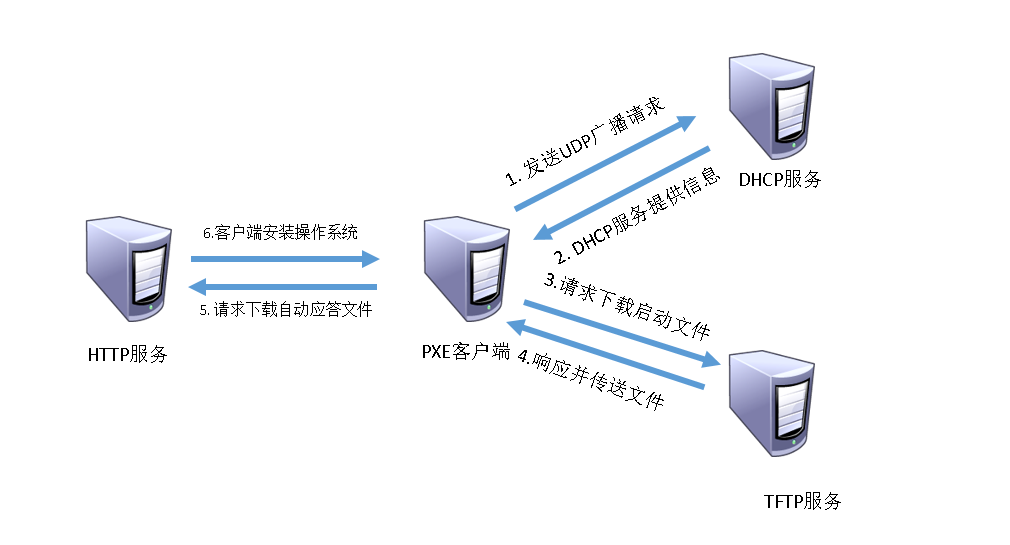
\includegraphics[width=0.8\textwidth]{./cobble/images/pxe-step.png}
\end{figure}

\begin{figure}[!ht]
    \centering
     \caption{\label{Fig:kickstart-dhcp} pxe step}
    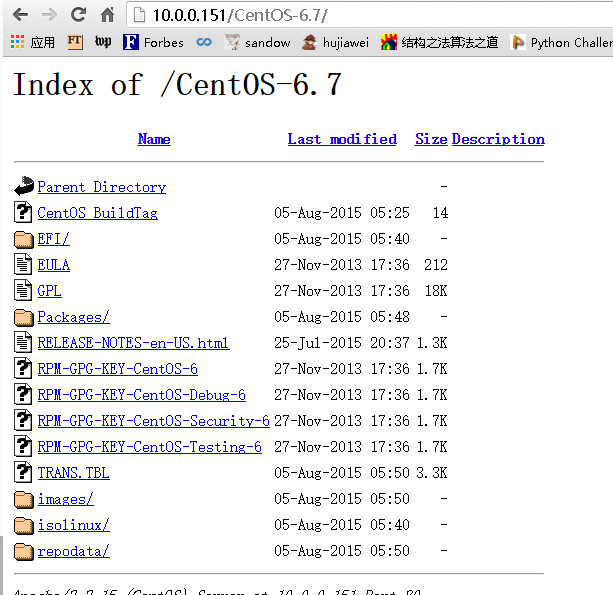
\includegraphics[width=0.8\textwidth]{./cobble/images/kickstart-dhcp.png}
\end{figure}

kickstart https://access.redhat.com/documentation/en-us/red_hat_enterprise_linux/6/html/installation_guide/s1-kickstart2-options


https://github.com/webdevops/Dockerfile.git
\chapter{docker基础到kubernetes集群}

\section{docker基础}

在gpu-docker使用
https://github.com/NVIDIA/nvidia-docker

\section{dockerfile 使用总结}

使用dockerfile 心得体会

\subsection{copy 和 add的区别}

COPY <src> <dest>

add 和 copy 都会把 src下面的复制到镜像中。例如 \textbf{COPY data /tmp } 便会把data下面的文件copy到/tmp下,
如果想把整个目录都复制过去那么就必须写成\textbf{COPY data /tmp/data } 这里copy和 add是一样的

虽然他们两功能非常像,在官方文档中的best practices for writing dockerfile时还是推荐使用copy

Although ADD and COPY are functionally similar, generally speaking, COPY is preferred. That’s because it’s more transparent than ADD. COPY only supports the basic copying of local files into the container, while ADD has some features (like local-only tar extraction and remote URL support) that are not immediately obvious. Consequently, the best use for ADD is local tar file auto-extraction into the image,

Because image size matters, using ADD to fetch packages from remote URLs is strongly discouraged; you should use curl or wget instead. That way you can delete the files you no longer need after they’ve been extracted and you won’t have to add another layer in your image.



\subsection{ENTRYPOINT 和 CMD}

docker并不会快照运行的进程,所以通过RUN命令运行的命令仅在 \textbf{docker build} 阶段的时候运行
如果需要在容器启动的时候运行服务需要使用ENTRYPOINT 和 CMD 来指定,并且这两命令都是放在dockerfile
的最后

并且 docker需要让进程一直处于running状态(前台,类似tail -F),也就是说不能运行在后台模式,不然docker会exit,并不会运行
除非特殊需求之外,一般一个容器只运行一个服务,也有时候需要运行多个服务,这时候可以有两种方法来解决,一是把两个服务
写到同一个shell里,然后运行,另一种便是使用supervisord,supervisord看起来是比较重的。

shell 示例

%\lstinputlisting{./scripts/run.sh}

supervisord 示例

\begin{lstlisting}[language=bash]
FROM ubuntu:latest
RUN apt-get update && apt-get install -y supervisor
RUN mkdir -p /var/log/supervisor
COPY supervisord.conf /etc/supervisor/conf.d/supervisord.conf
COPY my_first_process my_first_process
COPY my_second_process my_second_process
CMD ["/usr/bin/supervisord"]
\end{lstlisting}

ENTRYPOINT 会把docker run IMAGE 之外的所以参数都传给 ENTRYPOINT 执行的命令中。CMD则是完全覆盖
当ENTRYPOINT和CMD同时存在的时候 CMD会做为参数传给ENTRYPOINT。在docker run的时候如果有参数转进来,可以理解为覆盖CMD
然后把它做为参数传给ENTRYPOINT.
例如

\begin{lstlisting}[language=bash]
[root@ns1 test]# cat Dockerfile
FROM registry.gsandow.com:5043/centos
MAINTAINER from www.gsandow.com by sandow <j.k.yulei@gmail.com>

#ENTRYPOINT ["echo","entrypoit"]
CMD ["echo","cmd"]
[root@ns1 test]# docker build -t test .
Sending build context to Docker daemon  8.192kB
Step 1/3 : FROM registry.gsandow.com:5043/centos
 ---> 36540f359ca3
Step 2/3 : MAINTAINER from www.gsandow.com by sandow <j.k.yulei@gmail.com>
 ---> Using cache
 ---> c123904bd244
Step 3/3 : CMD echo cmd
 ---> Running in ea01464d732a
 ---> 3bcdf60c6bda
Removing intermediate container ea01464d732a
Successfully built 3bcdf60c6bda
Successfully tagged test:latest
[root@ns1 test]# docker run --rm test
cmd
[root@ns1 test]# docker run --rm test aaa
caused "exec: \"aaa\": executable file not found in \$PATH"
[root@ns1 test]# docker run --rm test echo aaa
aaa
[root@ns1 test]# cat Dockerfile
FROM registry.gsandow.com:5043/centos
MAINTAINER from www.gsandow.com by sandow <j.k.yulei@gmail.com>

ENTRYPOINT ["echo","entrypoit"]
CMD ["echo","cmd"]
[root@ns1 test]# docker build -t test .
[root@ns1 test]# docker run --rm test
entrypoit echo cmd
[root@ns1 test]# docker run --rm test echo 3
entrypoit echo 3
[root@ns1 test]# docker run --rm test cmd
entrypoit cmd
\end{lstlisting}

\noindent
Both CMD and ENTRYPOINT instructions define what command gets executed when running a container. There are few rules that describe their co-operation.

\smallskip
\begin{itemize}
	\item \small{Dockerfile should specify at least one of CMD or ENTRYPOINT commands.}
	\item \small{ENTRYPOINT should be defined when using the container as an executable.}
	\item \small{CMD should be used as a way of defining default arguments for an ENTRYPOINT command or for executing an ad-hoc command in a container.}
	\item \small{CMD will be overridden when running the container with alternative arguments.}

\end{itemize}

\noindent
The table below shows what command is executed for different ENTRYPOINT / CMD combinations:

\noindent
\begin{table}[h]
\begin{tabular*}{\textwidth}{|p{2.8cm}|p{3cm}|p{4cm}|p{5cm}|}
%\begin{tabular*}{0.7\paperwidth}{|l|l|l|l|}
	\hline
	&	No ENTRYPOINT &	ENTRYPOINT exec_entry p1_entry	& ENTRYPOINT [“exec_entry”, “p1_entry”] \\
	\hline
No CMD	&    error, not allowed & /bin/sh -c exec_entry p1_entry & exec_entry p1_entry \\
	\hline
CMD [“exec_cmd”, “p1_cmd”] & exec_cmd p1_cmd & /bin/sh -c exec_entry p1_entry & exec_entry p1_entry exec_cmd p1_cmd\\
	\hline
CMD [“p1_cmd”, “p2_cmd”] & p1_cmd p2_cmd & /bin/sh -c exec_entry p1_entry & exec_entry p1_entry p1_cmd p2_cmd \\
	\hline
CMD exec_cmd p1_cmd & /bin/sh -c exec_cmd p1_cmd & /bin/sh -c exec_entry p1_entry & exec_entry p1_entry /bin/sh -c exec_cmd p1_cmd \\
	\hline

\end{tabular*}
\end{table}

postgresql 官方例中ENTRYPOINT是这个样子的

\begin{lstlisting}
#!/bin/bash
set -e

if [ "$1" = 'postgres' ]; then
    chown -R postgres "$PGDATA"

    if [ -z "$(ls -A "$PGDATA")" ]; then
        gosu postgres initdb
    fi

    exec gosu postgres "$@"
fi

exec "$@"
\end{lstlisting}

	exec
	
	http://xstarcd.github.io/wiki/shell/exec_redirect.html

su,sudo 经常会需要TTY和信号转发行为,它们在设置和使用上比较。
gosu,便是在特定的用户下运行特定的程序然后退出管道。https://github.com/tianon/gosu

\section{docker 使用}

一般启动方式,以gitlab为例

\begin{lstlisting}[language=bash]
sudo docker run --detach \
    --hostname gitlab.example.com \
    --publish 443:443 --publish 80:80 --publish 22:22 \
    --name gitlab \
    --restart always \
    --volume /srv/gitlab/config:/etc/gitlab \
    --volume /srv/gitlab/logs:/var/log/gitlab \
    --volume /srv/gitlab/data:/var/opt/gitlab \
    gitlab/gitlab-ce:latest
\end{lstlisting}

\section{docker compose}

\begin{lstlisting}
web:
  image: 'gitlab/gitlab-ce:latest'
  restart: always
  hostname: 'gitlab.example.com'
  environment:
    GITLAB_OMNIBUS_CONFIG: |
      external_url 'http://gitlab.example.com:9090'
      gitlab_rails['gitlab_shell_ssh_port'] = 2224
  ports:
    - '9090:9090'
    - '2224:22'
  volumes:
    - '/srv/gitlab/config:/etc/gitlab'
    - '/srv/gitlab/logs:/var/log/gitlab'
    - '/srv/gitlab/data:/var/opt/gitlab'
\end{lstlisting}

docker-compose up -d


\section{参考链接}

\href{https://docs.docker.com/engine/userguide/eng-image/dockerfile_best-practices/}{dockerfile_best-practices}
\href{https://stackoverflow.com/questions/21553353/what-is-the-difference-between-cmd-and-entrypoint-in-a-dockerfile}{what-is-the-difference-between-cmd-and-entrypoint-in-a-dockerfile}
\href{https://stackoverflow.com/questions/24958140/what-is-the-difference-between-the-copy-and-add-commands-in-a-dockerfile}{what-is-the-difference-between-the-copy-and-add-commands-in-a-dockerfile}
\href{https://docs.docker.com/engine/admin/multi-service_container/}{ulti-service_container}


\section{kubernetes 组件及基础概念}

\href{ https://www.youtube.com/watch?v=_vHTaIJm9uY&list=PLF3s2WICJlqOiymMaTLjwwHz-MSVbtJPQ}{kubernetes 基础介绍视频链接}

\subsection{kube-master}

\begin{itemize}

	\item Kubernetes is highly api centered. The Kubernetes API server validates and configures data for the api objects which include pods, services, replicationcontrollers, and others. The API Server services REST operations and provides the frontend to the cluster’s shared state through which all other components interact.

        \item The Kubernetes scheduler is a policy-rich, topology-aware, workload-specific function that significantly impacts availability, performance, and capacity. The scheduler needs to take into account individual and collective resource requirements, quality of service requirements, hardware/software/policy constraints, affinity and anti-affinity specifications, data locality, inter-workload interference, deadlines, and so on. Workload-specific requirements will be exposed through the API as necessary.

        \item The Kubernetes controller manager is a daemon that embeds the core control loops shipped with Kubernetes. In applications of robotics and automation, a control loop is a non-terminating loop that regulates the state of the system. In Kubernetes, a controller is a control loop that watches the shared state of the cluster through the apiserver and makes changes attempting to move the current state towards the desired state. Examples of controllers that ship with Kubernetes today are the replication controller, endpoints controller, namespace controller, and serviceaccounts controller

\end{itemize}

The Kubernetes network proxy runs on each node. This reflects services as defined in the Kubernetes API on each node and can do simple TCP,UDP stream forwarding or round robin TCP,UDP forwarding across a set of backends. Service cluster ips and ports are currently found through Docker-links-compatible environment variables specifying ports opened by the service proxy. There is an optional addon that provides cluster DNS for these cluster IPs. The user must create a service with the apiserver API to configure the proxy.
 
The kubelet is the primary “node agent” that runs on each node. The kubelet works in terms of a PodSpec. A PodSpec is a YAML or JSON object that describes a pod. The kubelet takes a set of PodSpecs that are provided through various mechanisms (primarily through the apiserver) and ensures that the containers described in those PodSpecs are running and healthy. The kubelet doesn’t manage containers which were not created by Kubernetes.

Other than from an PodSpec from the apiserver, there are three ways that a container manifest can be provided to the Kubelet.
File: Path passed as a flag on the command line. Files under this path will be monitored periodically for updates. The monitoring period is 20s by default and is configurable via a flag.
HTTP endpoint: HTTP endpoint passed as a parameter on the command line. This endpoint is checked every 20 seconds (also configurable with a flag).
HTTP server: The kubelet can also listen for HTTP and respond to a simple API (underspec’d currently) to submit a new manifest.

fluentd is the component which is basically responsible for managing the logs and talking to the central locking mechanism

\subsection{kube-node}



\href{https://github.com/kubernetes/kops}{kops   安装,升级,管理工具}


flanneld

\begin{lstlisting}
/usr/lib/sysctl.d/00-system.conf
net.bridge.bridge-nf-call-iptables=1
net.bridge.bridge-nf-call-ip6tables=1
sysctl -w net.ipv4.ip_forward=1
sysctl -w net.bridge.bridge-nf-call-ip6tables=1
sysctl -w net.bridge.bridge-nf-call-iptables=1
\end{lstlisting}

0down vote	What parameters did you provide for kubeadm?
	If you want to use flannel as the pod network, specify --pod-network-cidr 10.244.0.0/16 if you’re using the daemonset manifest below. However, please note that this is not required for any other networks besides Flannel
	Execute these commands on every node:





\subsection{ pod}

pod is a group of one or more containers that are always co-located and
co-scheduled that share the context, containers in a pod share the same
IP address,ports,hostname, and storage. modeled like a virtual machine:
each container represnets one process
tightly coupled with other containers in the same pod

pod are scheduled in nodes, fundamental unit of deployment in kubernetes.

use cases for pod



\subsection{Replication Controller}

Ensures that a pod or homogeneous set of pods are always up and available
Always maintains desired number of pods
if there are exess pod, they get killed
new pods are launched when they fail, get deleted, or terminated

creating a replication controller with a count of 1 ensoures that a pod 
is always availble
RC and Pods are associated througth lables

\subsection{replica set}

replica set is the advancement to replication controller
replica sets are the nest generation Replication controller
ensures specified numbers of pods are always running
Pods are replaced by Replica Sets when a failure occurs
lables and selectors are useed for associating pods with replica set
usually combined with pods when defining the deployment


如果定义的pod,删除或者终止后不会重建,定义成RC后,删除或者终结后还会重建一个

kubectl scale rc web --replicas=20  
也可以这样来定制RC


separate statefull containers and stateless containers because stateful containers have very
stringent requirements for example i might want to have an SSD based storage that is mounted
as a volume 


\subsection{ Service}
a Service is an abstraction of a logical set of Pods defined by a policy
it acts as the intermediary for pods to talk to each other
selectors are used for accesing all the pods that match a specific lable
service is an object in kubernetes - similar to pods and RCs
each Service exposes one of more ports and targetPorts: port will expose to its consumers
the targetPorts is how it is going to route the traffic to the destination pods
The targetPort is mapped to the port exposed by matching Pods
Kubernetes Services Support TCP and UDP portocols


kubectl create -f pod.yml -f rc.yml 
kubectl create -f svc.yml

kubectl apply -f svc.yml


red, green, blue 可以分别定义开发,测试,正式环境,然后通过svc提供服务,只需要改变select便可以轻松切到某个环境

\section{kubectl高级用法}

kubectl 来获取特殊的值

\begin{lstlisting}

获取node name
 kubectl get nodes -o jsonpath='{range.items[*].metadata}{.name} {end}'

获取node ip
kubectl get nodes -o jsonpath='{range .items[*].status.addresses[?(@.type=="ExternalIP")]}{.address} {end}'

 一:get 过滤及格式化输出
kubectl get pods --all-namespaces -o jsonpath="{..image}"
kubectl get pods --all-namespaces -o jsonpath="{.items[*].spec.containers[*].image}"

    * .items[*]: for each returned value
    * .spec: get the spec
    * .containers[*]: for each container
    * .image: get the image
上面的一般都不会格式化输出,需要使用range来结合使用
kubectl get pods --all-namespaces -o=jsonpath='{range .items[*]}{"\n"}{.metadata.name}{":\t"}{range .spec.containers[*]}{.image}{", "}{end}{end}' 

Kubectl run my-web —image=nginx —port=80
Kubectl expose deployment my-web —target-port=80 —type=NodePort

Kubectl get svc my-web -o to-templates=‘{{(index .spec.ports 0).nodePort}}’

切到另一个集群
kubectl config view
kubectl config user-context xxxx
kubectl config use-context  xxxx

\end{lstlisting}




\section{定义pod}

\subsection{限制容器使用资源}

创建包含一个容器的Pod,这个容器申请100M的内存,并且内存限制设置为200M
放在contaner 下面

jkljl \cite{Survey2014}
\printbibliography

\begin{lstlisting}
    resources:
      limits:
        memory: "200Mi"
      requests:
        memory: "100Mi"
\end{lstlisting}


\subsection{pod生命周期与重启策略}

A pod (as in a pod of whales or pea pod) is a group of one or more containers (such as Docker containers), with shared storage/network, and a specification for how to run the containers. A pod’s contents are always co-located and co-scheduled, and run in a shared context. A pod models an application-specific “logical host” - it contains one or more application containers which are relatively tightly coupled — in a pre-container world, they would have executed on the same physical or virtual machine.

\href{https://kubernetes.io/docs/concepts/workloads/pods/pod/#termination-of-pods}{ermination-of-pods}

The kubelet can optionally perform and react to two kinds of probes on running Containers:

The kubelet uses liveness probes to know when to restart a Container. For example, liveness probes could catch a deadlock, where an application is running, but unable to make progress. Restarting a Container in such a state can help to make the application more available despite bugs.

The kubelet uses readiness probes to know when a Container is ready to start accepting traffic. A Pod is considered ready when all of its Containers are ready. One use of this signal is to control which Pods are used as backends for Services. When a Pod is not ready, it is removed from Service load balancers.

\begin{description}
\item[livenessProbe] Indicates whether the Container is running. If the liveness probe fails, the kubelet kills the Container, and the Container is subjected to its restart policy. If a Container does not provide a liveness probe, the default state is Success.
\item[readinessProbe] Indicates whether the Container is ready to service requests. If the readiness probe fails, the endpoints controller removes the Pod’s IP address from the endpoints of all Services that match the Pod. The default state of readiness before the initial delay is Failure. If a Container does not provide a readiness probe, the default state is Success
\end{description}

Probes have a number of fields that you can use to more precisely control the behavior of liveness and readiness checks:

\begin{description}
	\item[initialDelaySeconds] Number of seconds after the container has started before liveness or readiness probes are initiated.
	\item[periodSeconds] How often (in seconds) to perform the probe. Default to 10 seconds. Minimum value is 1.
	\item[timeoutSeconds] Number of seconds after which the probe times out. Defaults to 1 second. Minimum value is 1.
	\item[successThreshold] Minimum consecutive successes for the probe to be considered successful after having failed. Defaults to 1. Must be 1 for liveness. Minimum value is 1.
	\item[failureThreshold] When a Pod starts and the probe fails, Kubernetes will try failureThreshold times before giving up. Giving up in case of liveness probe means restarting the Pod. In case of readiness probe the Pod will be marked Unready. Defaults to 3. Minimum value is 1.
\end{description}

HTTP probes have additional fields that can be set on httpGet:

\begin{description}
	\item[host] Host name to connect to, defaults to the pod IP. You probably want to set “Host” in httpHeaders instead.
	\item[scheme] Scheme to use for connecting to the host (HTTP or HTTPS). Defaults to HTTP.
	\item[path] Path to access on the HTTP server.
	\item[httpHeaders] Custom headers to set in the request. HTTP allows repeated headers.
	\item[port] Name or number of the port to access on the container. Number must be in the range 1 to 65535.
For an HTTP probe, the kubelet sends an HTTP request to the specified path and port to perform the check. The kubelet sends the probe to the pod’s IP address, unless the address is overridden by the optional hostfield in httpGet. If scheme field is set to HTTPS, the kubelet sends an HTTPS request skipping the certificate verification. In most scenarios, you do not want to set the host field. Here’s one scenario where you would set it. Suppose the Container listens on 127.0.0.1 and the Pod’s hostNetwork field is true. Then host, under httpGet, should be set to 127.0.0.1. If your pod relies on virtual hosts, which is probably the more common case, you should not use host, but rather set the Host header in httpHeaders.
\end{description}

\href{https://kubernetes.io/docs/tasks/configure-pod-container/configure-liveness-readiness-probes/}{configure-liveness-readiness-probes}

A Probe is a diagnostic performed periodically by the kubelet on a Container. To perform a diagnostic, the kubelet calls a Handler implemented by the Container. There are three types of handlers:

\begin{description}
\item[ExecAction] Executes a specified command inside the Container. The diagnostic is considered successful if the command exits with a status code of 0.
\item[TCPSocketAction] Performs a TCP check against the Container’s IP address on a specified port. The diagnostic is considered successful if the port is open.
\item[HTTPGetAction] Performs an HTTP Get request against the Container’s IP address on a specified port and path. The diagnostic is considered successful if the response has a status code greater than or equal to 200 and less than 400.
\end{description}

Each probe has one of three results:
Success: The Container passed the diagnostic.
Failure: The Container failed the diagnostic.
Unknown: The diagnostic failed, so no action should be taken.

A PodSpec has a restartPolicy field with possible values Always, OnFailure, and Never. The default value is Always. restartPolicy applies to all Containers in the Pod. restartPolicy only refers to restarts of the Containers by the kubelet on the same node. Failed Containers that are restarted by the kubelet are restarted with an exponential back-off delay (10s, 20s, 40s …) capped at five minutes, and is reset after ten minutes of successful execution. As discussed in the Pods document, once bound to a node, a Pod will never be rebound to another node.


\href{https://kubernetes.io/docs/concepts/workloads/pods/pod-lifecycle/}{pod-lifecycle}

Kubernetes supports the postStart and preStop events. Kubernetes sends the postStart event immediately after a Container is started, and it sends the preStop event immediately before the Container is terminated

https://kubernetes.io/docs/tasks/configure-pod-container/attach-handler-lifecycle-event/
https://kubernetes.io/docs/concepts/containers/container-lifecycle-hooks/

\subsection{创建pod拉取私有库镜像}
拉取镜像由 imagePullPolicy 来控制拉取策略,他有三个值   Always IfNotPresent Never


当使用私有库拉镜像的时候需要创建secret 

kubectl create secret docker-registry myregistrykey --docker-server=DOCKER_REGISTRY_SERVER --docker-username=DOCKER_USER --docker-password=DOCKER_PASSWORD --docker-email=DOCKER_EMAIL
secret "myregistrykey" created.

使用yaml,来创建secret这时候有一点麻烦,需要先docker login 登录私钥库,可以看到在家目录多出来个.docker隐藏目录,下面有config.json文件,这时需要使用base64加密,在定义secrete 时需要把加密后的值连续的赋予给data[".dockerconfigjson"]

\begin{lstlisting}
docker login  -u admin -p Harbor123  10.10.39.226
[root@mobius_004 ~]# cd .docker/
[root@mobius_004 .docker]# ls
config.json
[root@mobius_004 .docker]# cat config.json
{
	"auths": {
		"10.10.39.226": {
			"auth": "YWRtaW46SGFyYm9yMTIzNDU="
		}
	},
	"HttpHeaders": {
		"User-Agent": "Docker-Client/18.01.0-ce (linux)"
	}
}
[root@mobius_004 .docker]# base64EncodeData=$(base64 -w 0 config.json)
[root@mobius_004 .docker]# echo $base64EncodeData|base64 --decode
apiVersion: v1
kind: Secret
metadata:
  name: myregistrykey
  namespace: awesomeapps
data:
  .dockerconfigjson: $base64EncodeData

type: kubernetes.io/dockerconfigjson

然后在创建pod的时候指定secrets来拉镜像

apiVersion: v1
kind: Pod
metadata:
  name: foo
  namespace: awesomeapps
spec:
  containers:
    - name: foo
      image: janedoe/awesomeapp:v1
  imagePullSecrets:
    - name: myregistrykey

\end{lstlisting}

https://kubernetes.io/docs/concepts/containers/images/

\section{kubeconfig 配置}

kubeconfig 在kubectl, kubelet, kube-proxy,bootstrap都会用到,配置kubeconfig可以用三种方式

通过命令方式

\begin{lstlisting}
 kubectl config set-cluster kubernetes \
  --certificate-authority=/etc/kubernetes/ssl/ca.pem \
  --embed-certs=true \
  --server=${KUBE_APISERVER} \
  --kubeconfig=kube-proxy.kubeconfig
 # 设置客户端认证参数
 kubectl config set-credentials kube-proxy \
  --client-certificate=/etc/kubernetes/ssl/kube-proxy.pem \
  --client-key=/etc/kubernetes/ssl/kube-proxy-key.pem \
  --embed-certs=true \
  --kubeconfig=kube-proxy.kubeconfig
 # 设置上下文参数
 kubectl config set-context default \
  --cluster=kubernetes \
  --user=kube-proxy \
  --kubeconfig=kube-proxy.kubeconfig
 # 设置默认上下文
 kubectl config use-context default --kubeconfig=kube-proxy.kubeconfig
 mv kube-proxy.kubeconfig /etc/kubernetes/
\end{lstlisting}

直接编辑方式

.kube/config 这个配置文件可以指定文件或者指定base64值


\begin{lstlisting}
apiVersion: v1
kind: Config
users:
- name: kubelet
  user:
    client-certificate-data: <base64-encoded-cert>
    client-key-data: <base64-encoded-key>
clusters:
- name: local
  cluster:
    certificate-authority-data: <base64-encoded-ca-cert>
contexts:
- context:
    cluster: local
    user: kubelet
  name: service-account-context
current-context: service-account-context

\end{lstlisting}

加密密钥可以使用 base64 /Users/yulei/Documents/ansible/roles/kubernetes/files/ssl/ca.pem 便可得到

To generate the base64 encoded client cert, you should be able to run something like cat /var/run/kubernetes/kubelet_36kr.pem | base64. If you don't have the CA certificate handy, you can replace the certificate-authority-data: <base64-encoded-ca-cert> with insecure-skip-tls-verify: true.

If you put this file at /var/lib/kubelet/kubeconfig it should get picked up automatically. Otherwise, you can use the --kubeconfig argument to specify a custom location.

或者在config里指定文件

apiVersion: v1
clusters:
- cluster:
    certificate-authority: /etc/kubernetes/certs/ca.crt
    server: https://kubernetesmaster
  name: default-cluster
contexts:
- context:
    cluster: default-cluster
    user: default-admin
  name: default-system
current-context: default-system
kind: Config
preferences: {}
users:
- name: default-admin
  user:
    client-certificate: /etc/kubernetes/certs/server.crt
    client-key: /etc/kubernetes/certs/server.key


\section{生产环境中使用kubernetes}

Kubernetes in prod

https://techbeacon.com/one-year-using-kubernetes-production-lessons-learned

https://github.com/kelseyhightower/confd

https://www.graylog.org/

https://www.loggly.com/blog/top-5-docker-logging-methods-to-fit-your-container-deployment-strategy/

https://medium.com/readme-mic/kubernetes-1-year-in-production-f406bdb95c22

https://kubernetes.io/docs/reference/generated/kubernetes-api/v1.9/


https://blog.dockbit.com/kubernetes-canary-deployments-for-mere-mortals-6696910a52b2

https://kubernetes.io/docs/concepts/overview/what-is-kubernetes/

https://www.loggly.com/resource/log-management-handbook-docker/

https://medium.com/readme-mic/kubernetes-1-year-in-production-f406bdb95c22


https://medium.com/readme-mic/kubernetes-1-year-in-production-f406bdb95c22

\subsection{openshift}

https://github.com/openshift/origin

http://www.linkedin.com/pulse/part-2-kubernetes-services-minikube-docker-james-denman


学习集群

https://www.katacoda.com/courses/kubernetes/playground


\section{kubernetes addon}


\subsection{Discovering Services}
discovering services - dns
the DNS server watches kubernetes API for new Services
the DNS server creates a set of DNS recordes for each Services
Services can be resolved by the name within the same namespace
Pods in other namespaces can access the Service by adding the namespace to the DNS path
  my-service.my-namespace

Discovering Services - env vars

Service Types
 ClusterIP: service is reachable only from inside of the cluster
NodePort
 Service is reachable through NodeIP:NodePort address
LoadBalancer
  service is reachable through an external load balancer mapped to NoderIP:NodePort address

kubernetes create Docker link compatible environment variables in all pods
containers can use the environment variable to talk to the service endpoint

https://segmentfault.com/a/1190000002892825


\section{pod的持久化}

persistence in pods

pods are ephemeral and stateless

volumes bring persistence to pods

kubernetes voluems are similar to docker volumes, but managed differently

all containers in pod can access the volumes

volumes are associated with the lifecycle of pod

directories in the host are exposed as volumes

volumes may be based on a variety of storage backends

kubernetes have three method to persistence into your workload

1:  basic volume will persistence to you pod with from limitations
2: rely on distributed storage like NFS
3: clear dispersing,

kubernetes volume types

\begin{lstlisting}
- hostbased
   emptydir
    hostpath
- block storage
  amazon EBS
  GCE Psersistent Disk
  Azure Disk
  VSphere Volume
- Distributed file System
  NFS
  Ceph
  Gluster
  Amazon EFS
- other
  Flocker
  iScsi
  Git Repo



gcloud container clusters get-credentials jani-gke-demo asia-east1-a
gcloud compute disks create --size=10G --zone=asia-east1-a my-data-disk
gcloud compute disks delete --zone=asia-east1-a my-data-dis

\end{lstlisting}


Unserstanding Psersistent Volume and Claims

PersistentVolume(PV)
  Networked storage in ther cluster per-provisioned  by a administrator
PersistentVolumeClaim (PVC)
  Storage resource requested by a user.
StorageClass
  types of supported storage profiles offered by administrator




%\part{linux 基础知识}

在第一部门中先了解linux基础操作知识,他们包括系统知识,网络知识,


\chapter{系统基础}

\section{centos7 安装}

CentOS 7 网卡名不以eth0开始原因,是由于systemd 和 udev 引入了一种新的网络设备命名方式–一致网络设备命名(CONSISTENT NETWORK DEVICE NAMING) 。可以根据固件、拓扑、位置信息来设置固定名字,带来的好处是命名自动化,名字完全可预测,在硬件坏了以后更换也不会影响设备的命名,这样可以让硬件的更换无缝化。带来的不利是新的设备名称比传统的名称难以阅读。比如心得名称是enp5s0.

想要改为像centos6一样以eth0开始的名称有两种方法,在出现安装新系统的时候按下tab键,在kernel启动选项中增加 net.ifnames=0 biosdevname=0 


\begin{figure}[!ht]
    \centering    
     \caption{\label{Fig:async} Asynchronous I/O model}
    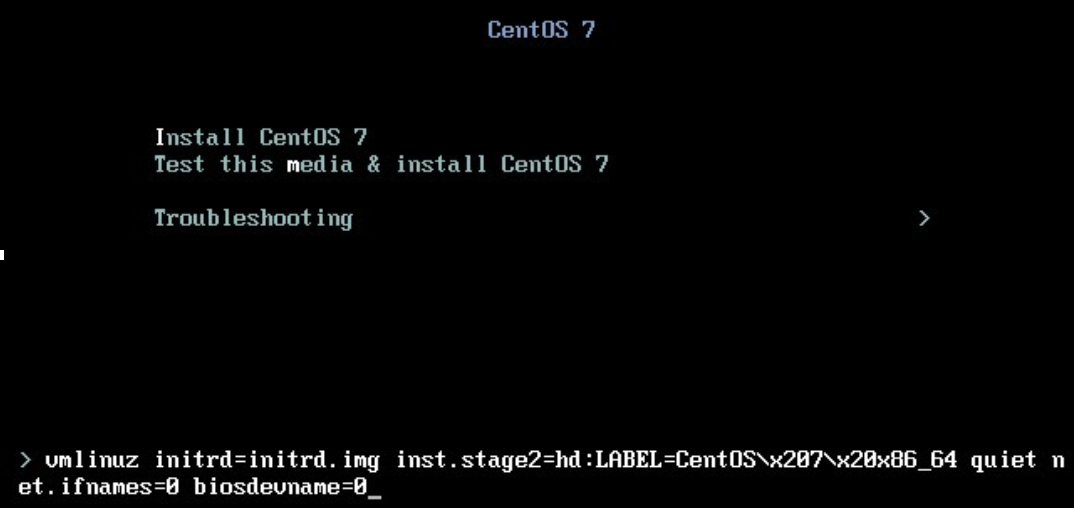
\includegraphics[width=0.8\textwidth]{./images/centos-bios.png}  
\end{figure}

当然,如果在安装时忘记操作了也可以在启动后操作。在 /etc/sysconfig/grub下相应位置加上这两个参数,然后再改网卡名既可

\begin{lstlisting}
GRUB_CMDLINE_LINUX=”rd.lvm.lv=vg0/swap vconsole.keymap=us crashkernel=auto  vconsole.font=latarcyrheb-sun16 net.ifnames=0 biosdevname=0 rd.lvm.lv=vg0/usr rhgb quiet”

grub2-mkconfig -o /boot/grub2/grub.cfg

\end{lstlisting}

安装完系统后一般需要关闭selinux, NetworkManager, firewalld, 需要安装net-tools, lsof, tcpdump, epel,

\subsection{桥接}

一、网卡桥接设置:

1、网卡配置文件:

[root@localhost /]# vim /etc/sysconfig/network-scripts/ifcfg-enp8s0

TYPE=Ethernet
DEVICE=enp8s0
NAME=enp8s0
BOOTPROTO=none
ONBOOT=yes
BRIDGE=br0

 2、网桥配置文件:

[root@localhost /]# vim /etc/sysconfig/network-scripts/ifcfg-br0

TYPE=Bridge
DEVICE=br0
BOOTPROTO=static
ONBOOT=yes
IPADDR=192.168.1.200
NETMASK=255.255.255.0
GATEWAY=192.168.1.1
DNS1=114.114.114.114


二、网卡绑定设置:

1、网卡配置文件01:

[root@localhost /]# vim /etc/sysconfig/network-scripts/ifcfg-enp6s0f0

TYPE=Ethernet
DEVICE=enp6s0f0
NAME=enp6s0f0
BOOTPROTO=none
ONBOOT=yes
USERCTL=no
MASTER=bond0
SLAVE=yes
2、网卡配置文件02:

[root@localhost /]# vim /etc/sysconfig/network-scripts/ifcfg-enp6s0f1

TYPE=Ethernet
DEVICE=enp6s0f1
NAME=enp6s0f1
BOOTPROTO=none
ONBOOT=yes
USERCTL=no
MASTER=bond0
SLAVE=yes
3、网桥配置文件:

[root@localhost /]# vim /etc/sysconfig/network-scripts/ifcfg-bond0

TYPE=Ethernet
DEVICE=bond0
BOOTPROTO=static
ONBOOT=yes
USERCTL=no
IPADDR=172.16.1.216
NETMASK=255.255.255.0
GATEWAY=172.16.1.1
DNS1=114.114.114.114

3. 在bond0基础上增加多个桥接网卡
[root@yw-qa-kvm-04 network-scripts]# cat ifcfg-bond0.300
BOOTPROTO=none
DEVICE=bond0.300
ONBOOT=yes
VLAN=yes
BRIDGE=virbr300
[root@yw-qa-kvm-04 network-scripts]# cat ifcfg-bond0.3960
BOOTPROTO=none
DEVICE=bond0.3960
ONBOOT=yes
VLAN=yes
BRIDGE=virbr3960

[root@yw-qa-kvm-04 network-scripts]# cat ifcfg-virbr300
TYPE=bridge
BOOTPROTO=static
DEVICE=virbr300
ONBOOT=yes
IPADDR=10.30.0.252
NETMASK=255.255.255.0
DELAY=0
[root@yw-qa-kvm-04 network-scripts]# cat ifcfg-virbr3960
TYPE=bridge
BOOTPROTO=static
DEVICE=virbr3960
ONBOOT=yes
IPADDR=10.18.61.252
NETMASK=255.255.255.0
DELAY=0


\section{磁盘分区与挂载}

\subsection{磁盘简介}
用于存储数据的物理设备便叫磁盘,磁盘接接口的不同可以分为:IDE,  SATA, SCSI, SAS.

\begin{itemize}
\item IDE的英文全称为“Integrated Drive Electronics”,即“电子集成驱动器”,
\item SCSI的英文全称为“Small Computer System Interface”
\item SATA(Serial ATA)又叫串口硬盘,PC机硬盘的主流趋势。
\item SAS(Serial Attached SCSI)即串行连接SCSI,是新一代的SCSI技术,此接口的设计是为了改善存储系统的效能、可用性和扩充性,并且提供与SATA硬盘的兼容性
\end{itemize}

磁盘内部由多个盘片,机械手臂,磁头,主轴马达组成。在读取数据时主轴马达驱动盘片转动,机械手臂可伸展来让磁头(head)读取数据,在盘片上存储数据,所以磁盘的容量便要看盘片的质量。

\begin{description}
	\item[磁道(Track)]:在每个盘片上由不同半经组成的同心圆叫做磁道,
	\item]扇区(Sector)]:每个磁道中被分隔成的最小的俱单位便是扇区每个扇区为512bytes
	\item[柱面(Cylinder)]:由多个盘片相同磁道所组成的圆柱面便是柱面
\end{description}

磁盘读取与写入数据时会按柱面来写入,只有柱面写完(读完)后才会切换磁道。
磁盘容量计算方式:Head * cylinder * Secor * 512bytes

每个磁盘的第一扇区非常重要,因为在该扇区存放着两个重要信息
1. 主引导分区(Master Boot Record, MBR) 有446bytes 主要用于安装引导加载程序
2. 分区表(Partition table) 记录整块磁盘分区状态,有64bytes

\subsection{磁盘分区}
由于分区表仅有64bytes所以只能记录4组记录区,每组记录区记录了该区段的启始与结束的柱面号码。所以每个磁盘只能分四个主(Primary)或扩展分区(Extended)。
而每个磁盘只允许有一个扩展分区,且扩展分区不能被格式化后存放数据,需要在扩展分区之上划分逻辑分区(Logical)。linux设备中的文件名1-4给主或者扩展分区预留,逻辑分区从5开始。

在linux下给磁盘分区的命令有`fdisk` 适合小于2T的磁盘分区, `parted` 擅长于大于2t 的磁盘分区。分区的实质便是修改分区表

\subsubsection{ fdisk 对磁盘分区}
使用命令`fdisk -cu /dev/sdb` 来进行对sdb分区,用命 -l来查看分区分区时的命令有

\begin{itemize}
\item  d   delete a partition 删除一个分区
\item  n   add a new partition       新增一个分区
\item  p   print the partition table 把分区打印出来
\item  q   quit without saving changes 不保存退出
\item  w   write table to disk and exit  保存分区并退出
\end{itemize}

这里需要注意在交互式分区过程中输错之后需要用**Ctrl + u**来撤消。 交互式实在太费事,这对于批量分区来说太费事可以用下面命令来一键搞定
\begin{lstlisting}
echo -e "n\np\n1\n\n+10G\nn\np\n2\n\n+20G\nw" |fdisk /dev/sdb
\end{lstlisting}

上一便仅是创建两个主分区,第一个分区给10G,第二个分区给20G,创建其它分区也类似

\subsubsection{ parted 对磁盘分区}
parted的操作都是实时的,也就是说你执行了一个分区的命令,他就实实在在地分区了,而不是像fdisk那样,需要执行w命令写入所做的修改, 所以进行parted的测试千万注意不能在生产环境中!
>传统的MBR(Master Boot Record)分区方式,有一个局限:无法支持超过2TB的硬盘的分区(或单个分区超过2TB)如果大于2T就要使用用GPT(Globally Unique Identifier Partition Table Format)分区的概念.

非交互式分区方式

\begin{lstlisting}
parted /dev/sdb  mklabel gpt yes
parted /dev/sdb  mkpart primary ext4 0 100  Ignore
parted /dev/sdb  mkpart primary linux-swap 101 8192 Ignore
parted /dev/sdb  mkpart logical ext4 8193 100GB  Ignore
parted /dev/sdb  mkpart logical ext4 101GB 3000GB Ignore
parted /dev/sdb  quit
\end{lstlisting}

\subsection{ 格式化与挂载}
磁盘分区好后,必须先格式化后才能挂载

\begin{lstlisting}
$ mkfs.ext4 /dev/sdb1
$ mkfs.ext4 /dev/sdb2

$ tune2fs -c -1 /dev/sdb1
tune2fs 1.41.12 (17-May-2010)
Setting maximal mount count to -1
#格式化后便可以挂载了
$ mount /dev/sdb1 /mnt
$ mount |grep --color=auto "/dev/sdb1"
/dev/sdb1 on /mnt type ext4 (rw)
\end{lstlisting}

在这里手动挂载后,系统重启后还需要再手动挂载一次,因为这里需要修改文件/etc/fstab 这个文件以达到开机自动挂载

磁盘被手动挂载之后都必须把挂载信息写入/etc/fstab这个文件中,否则下次开机启动时仍然需要重新挂载。 系统开机时会主动读取/etc/fstab这个文件中的内容,根据文件里面的配置挂载磁盘。这样我们只需要将磁盘的挂载信息写入这个文件中我们就不需要每次开机启动之后手动进行挂载了。挂载的限制
\begin{itemize}
\item  根目录是必须挂载的,而且一定要先于其他mount point被挂载。因为mount是所有目录的跟目录,其他木有都是由根目录 /衍生出来的。
\item  挂载点必须是已经存在的目录。
\item  挂载点的指定可以任意,但必须遵守必要的系统目录架构原则
\item  所有挂载点在同一时间只能被挂载一次
\item  所有分区在同一时间只能挂在一次
\item  若进行卸载,必须将工作目录退出挂载点(及其子目录)之外。
\end{itemize}

下面我们看看看/etc/fstab文件,这是我的linux环境中/etc/fstab文件中的内容

\begin{lstlisting}[language=bash]

$ cat /etc/fstab

#
# /etc/fstab
# Created by anaconda on Wed Oct 28 23:23:38 2015
#
# Accessible filesystems, by reference, are maintained under '/dev/disk'
# See man pages fstab(5), findfs(8), mount(8) and/or blkid(8) for more info
#
UUID=faba0886-9c24-430c-8ce5-f7980c283bbd /                       ext4    defaults        1 1
UUID=a2ea9c91-9424-4d8e-b15f-946ef8413877 /boot                   ext4    defaults        1 2
UUID=f11549e2-cd8a-4ec5-92ca-e8a83a16c87e swap                    swap    defaults        0 0
tmpfs                   /dev/shm                tmpfs   defaults        0 0
devpts                  /dev/pts                devpts  gid=5,mode=620  0 0
sysfs                   /sys                    sysfs   defaults        0 0
proc                    /proc                   proc    defaults        0 0
/dev/sdb1               /mnt                    ext4    defaults        0 0

\end{lstlisting}

可以看到fstab里一共有六列。

第一列 Device **Device**  是磁盘设备文件或者该设备的Label或者UUID
Label就是分区的标签,在最初安装系统是填写的挂载点就是标签的名字。可以通过查看一个分区的superblock中的信息找到UUID和Label name。
例如我们要查看/dev/sda1这个设备的uuid和label name
使用设备名称(/dev/sda)来挂载分区时是被固定死的,一旦磁盘的插槽顺序发生了变化,就会出现名称不对应的问题。因为这个名称是会改变的。不过使用label挂载就不用担心插槽顺序方面的问题。不过要随时注意你的Label name。至于UUID,每个分区被格式化以后都会有一个UUID作为唯一的标识号。使用uuid挂载的话就不用担心会发生错乱的问题了。

\begin{lstlisting}[language=bash]
$ dumpe2fs -h /dev/sda1
dumpe2fs 1.35 (28-Feb-2004)
Filesystem volume name:   /boot   #这个就是Label name
Last mounted on:
Filesystem UUID:          3b10fe13-def4-41b6-baae-9b4ef3b3616c    #UUID
Filesystem magic number:  0xEF53
Filesystem revision #:    1 (dynamic)
Filesystem features:      has_journal ext_attr resize_inode dir_index filetype needs_recovery sparse_super
Default mount options:    (none)
Filesystem state:         clean
#简单点的方式我们可以通过下面这个命令来查看
$ blkid /dev/sda1
/dev/sda1: LABEL="/boot" UUID="3b10fe13-def4-41b6-baae-9b4ef3b3616c" SEC_TYPE="ext3" TYPE="ext2"
\end{lstlisting}


第二列:Mount point 设备的挂载点,就是你要挂载到哪个目录下。

第三列: filesystem 磁盘文件系统的格式,包括ext2、ext3、ext3、reiserfs、nfs、vfat等. 生产场景中如果是大量小文件业务 首选 reiserfs。而 ext4 适合视频下载,流媒体,数据库,小文件业务

 ReiserFS是一个基于B状树的文件系统,拥有非常好的总体性能,特别是对于大量小文件。ReiserFS 拥有良好的伸缩性并具有日志功能。但该文件系统不再受到积极开发,不支持SELinux,基本上已被 Reiser4 取代。ReiserFS文件系统多年来一直用作一些发行版(包括SUSE)的默认文件系统,但现在用得少了。

 XFS文件系统拥有日志功能,包含一些健壮的特性,并针对可伸缩性进行了优化。XFS在RAM中强制缓存中转数据,因此如果使用 XFS,建议采用不间断电源供应。淘宝的数据库在使用此文件系统。

第四列:parameters 文件系统的参数

\begin{description}
	\item[Async/sync]设置是否为同步方式运行,默认为async
	\item[auto/noauto]当挂载mount -a 的命令时,此文件系统是否被主动挂载。默认为auto
	\item[rw/ro      ]是否以以只读或者读写模式挂载
	\item[exec/noexec]限制此文件系统内是否能够进行"执行"的操作
	\item[user/nouser]是否允许用户使用mount命令挂载
	\item[suid/nosuid]是否允许SUID的存在
	\item[Usrquota	]启动文件系统支持磁盘配额模式
	\item[Grpquota	]启动文件系统对群组磁盘配额模式的支持
	\item[Defaults	]同事具有rw,suid,dev,exec,auto,nouser,async等默认参数的设置
\end{description}

第五列:能否被dump备份命令作用, dump是一个用来作为备份的命令。通常这个参数的值为0或者1, 0代表不要做dump备份, 1代表要每天进行dump的操作, 2 代表不定日期的进行dump操作

第六列 是否检验扇区 开机的过程中,系统默认会以fsck检验我们系统是否为完整(clean). 0 不要检验,1 最早检验(一般根目录会选择),2 1级别检验完成之后进行检验


 以上会用到的命令会另一篇文章专门介绍下面仅罗列一些相关的命令
\begin{description}
	\item[格式]:mkfs, tune2fs, dumpe2fs
	\item[挂载]: mount umount /etc/fstab
	\item[磁盘检查], df, fsck,  e2fsck
	\item[调整文件大小] resize2fs
	\item[分区]: fdisk parted, partprobe, dd
\end{description}


 给swap增加容量

\begin{lstlisting}[language=bash]
dd if=/dev/zero  of=/tmp/swap bs=1M count=128
mkswap  /tmp/swap
swapon  /tmp/swap
\end{lstlisting}


机械磁盘读写磁盘数据的原理小结:
1. 磁盘是按照柱面为单位读写数据的, 既先读取同一个盘面的某一个磁道,读完之后如果数据没有读完,磁头也不会切换到其他
的磁道, 而是选择切换磁头,读取下一个盘面相同半径的磁道, 直到所有盘面的相同半径的磁道读取完成之后,如果数据还没有读写成,才会切换其他不同半径的磁道,这个切换磁道的过程称为寻道。
2. 不同磁头间的切换是电子切换, 而不同磁道间的切换需要磁头做径向动动,这个径向运动需要不进行电机调节,这个运行是机械的切换。

第一个硬盘   第二个硬盘  第三个硬盘 , 使用硬件RAID, LVM等工成一个或者多个虚拟磁盘,在系统中以块设备名体现/dev/sda

/dev/sdb  等, 在进行使用之前需要进行格式化(创建虚拟文件系统,不同系统使用的文件系统不一样,xfs,ext3,ext4),每一个分区都有各自的inode与block.以供系统使用。

英文单词, Head磁头, Sector扇区, Track 磁道,Cylinder柱面,Units单元块, Block数据块, Inode索引节点
buffer: 一般 用于写操作, 写缓冲

Raid0是条带化,把多个磁盘合起来组成一个大磁盘 支持1 块到多块盘,容量是所有磁盘之和,读写速度最快,没有冗余
Raid1 只支持偶数盘,镜像盘。 读写性能一般,成本高
Raid5 奇偶校验盘,最少三块,可以块一块盘,写入恨不能不高
Raid10,先做Raid1然后再做Raid0,保存备份以及数据量,最少4块盘,读写性能快,成本高。


\section{文件描述符及通配符}

\subsection{ 通配符}
  普通命令都可以用的特殊符号,不同的通配符有不同的意义,现在简单介绍在linux中不同的通配符的不同意义。

|符号  |意义   |符号  |意义    |符号  |意义|
|:----|:------|:----|:------|:----|:-----|
|*     |所有   |?     | 代表一个字符|; |命令分隔符|
|#     |注释   |竖线  |  管道 |~ | 用户家目录|
|-     |上一次目录|  $|  调用变量| /|  路径分隔符|
|>  >> |重定向,追加重定向|<  <<| 输入重定向,追加输入重定向|{}    |内容序列|
|'     |无变量转换功能    |"    |里面变量可以转换| `(反引号) | 把里面内容当做命令执行|

简单举例

	mkdir /etc/{bbc, blog}
	echo {a..z}

	a=1
	printf "$a\n"     #输出是1
	printf '$a\n'     #输出结果是 $a
	echo `date`       #输出结果是当时时间长格式


i_link 硬链接
i_count 进程


删除 文件需要看所在目录是否有写权限,没有写权限时是无法删除目录下面的文件

\section{文件权限}
chmod  只有文件的属主或root 才能来改变文件权限。

创建目录默认755
创建文件默认644

umask  修改默认权限通过八进制的数值来定义用户 创建文件或目录的默认权限

sed -n '65.69p' /etc/bashrc

666-umask
若umask部分位为基数,那么在结果的相应位置加一

777-umask

umask 对应数值表示的是禁止的权限,


特殊权限位(用户权限位)

以下内容不重要:

suid   s(x)    S 4
sgid   s(x)    S 2
sticky t(x)    T 1  沾滞位只能用ROOT来删除或创建。被创建的目录,任何用户可以在该目录下可以创建文件目录,但不能查看其它用户的内容,(/tmp)

授权方法 chmod (4000|2000|1000) /bin/rm  chmod (u|g|o)+(s|t )


seuid  权限位
当二进制命令执行
修改的是命令而非文件
仅对二进制命令才有作用。
suid权限仅在程序命令执行过程中有效。
suid是比较危险的功能,

sgid 是针对用户 组权限位的
对文件来说,sgid的功能如下

sgid 仅对二进制的命令程序有效
二进制命令或程序需要有可执行权限
执行命令在任意用户 可以获得该命令程序执行期间所属组的权限。

sgid 针对 目录
创建一个目录,要求在其 目录下创建的文件或目录的group继承该目录组
chmod 2755 /home/admins/


设置seuid
chmod 4755 /bin/rm

find / -perm 4755 -type f



更改文件属主与组 chown  chgrp


chown owrner:group   dirctory|file
chown :group       dirctory|file
chown owrner       dirctory|file

 groupadd test -g 501


\section{shell}
可执行文件开头第一行一般我们会指定用什么解释器来执行该文件比如shell角本的文件开头一般会加`#! /bin/sh`
如果是python文件(后缀名为.py)在第一行增加 `#! /usr/bin/python`

{toc}

### shell定义变量以及调用变量

运行shell 时会遇到三种变量
1. 局部变量, 在脚本或命令中定义,仅在当前shell实例中有效,其他shell启动的程序不能访问局部变量。
2. 环境变量,  所有的程序,包括shell启动的程序,都能访问环境变量,有些程序需要环境变量来保证其正常运行。必要的时候shell脚本也可以定义环境变量。
3. shell变量, 是由shell程序设置的特殊变量。shell变量中有一部分是环境变量,有一部分是局部变量,这些变量保证了shell的正常运行

定义变量时,变量名开始必须以[a-zA-Z]开始,中间不可以有空格或标点符号(可以用“\_”),变量名不可以使用bash的关键字。
调用变量,只需要在变量名前加"$"便可以了,考虑到解释器识别边界的问题,一般我们会在变量名外加大括号来确定变量名
删除变量可以用 `unset` 来取消变量的定义 .

现在我们便创建一个test.sh文件并且给它执行权限在里面输入以下内容

```
#! /bin/sh

#变量定义举例:
myName="sandow"
myUrl="http://magdre.github.io"
myAge=34
#调用变量
echo "hell everyone my name is $myName, my blog site is $myUrl,"
echo "Today, I'm ${myAge}years old"
#删除变量
unset myName
```


大括号(花括号)是为了让解释器识别变量名的边界,如果不加的话变量名就成了 $myAgeyears 这个变量名为空,输出来的便只有 **Todey, I'm old**  这样与期望值并不一样。

---

#### 在shell中的特殊变量名


|变量|  含义 |
|:--:|:----|
|\$0  | 当前脚本的文件名 |
|\$n  |传递给脚本或函数的参数。n 是一个数字,表示第几个参数,例 `$1` 。 如果超过10便需要写成 `${10}`|
|\$#  |传递给脚本或函数的参数个数。 |
|\$*  |传递给脚本或函数的所有参数。 |
|\$@  |传递给脚本或函数的所有参数。被双引号(" ")包含时,与 \$* 稍有不同,下面将会讲到。 |
|\$?  |上个命令的退出状态,或函数的返回值。 |
|\$$  | 当前Shell进程ID。对于 Shell 脚本,就是这些脚本所在的进程ID。 |

现在我们接着在test.sh里输下面内容

```
echo "File Name: $0"
echo "First Parameter : $1"
echo "Second Parameter : $2"
echo "Quoted Values: $@"
echo "Quoted Values: $*"
echo "Total Number of Parameters : $#"
```
我们在命令行输入
```
$ ./test.sh hello world
```
便可以得到下面结果
```
./tesh.sh
hello
world
hello world
hello world
2
```

#### 变量赋值与转换


|形式  |说明|
|:---|:----|
|\${var} | 变量本来的值 |
|\${var:-word} | 如果变量 var 为空或已被删除(unset),那么返回 word,但不改变 var 的值。 |
|\${var:=word} | 如果变量 var 为空或已被删除(unset),那么返回 word,并将 var 的值设置为 word。 |
|\${var:?message} | 如果变量 var 为空或已被删除(unset),那么将消息 message 送到标准错误输出,可以用来检测变量 var 是否可以被正常赋值。 若此替换出现在Shell脚本中,那么脚本将停止运行。 |
|\${var:+word} | 如果变量 var 被定义,那么返回 word,但不改变 var 的值。 |

#### shell里的运算
在原生bash中不支持简单的数学运算,但是可以通过其他命令来实现,例如 awk 和 expr,expr 最常用。
在使用expr时的格式为 `expr 1 + 2 `

a=10
b=20

**算术运算符**

|运算符 |说明 | 举例 |
|:--:|:--:|:---|
|\+   |加法 |`expr $a + $b` 结果为 30。|
|\-   |减法 |`expr $a - $b` 结果为 10。|
|\*   |乘法 |`expr $a \* $b` 结果为  200。|
|\/   |除法 |`expr $b / $a` 结果为 2。 |
|%   |取余 |`expr $b % $a` 结果为 0。 |
|=   |赋值 | a=\$b 将把变量 b 的值赋给 a。 |
|== |相等 |用于比较两个数字,相同则返回 true。 \[ $a == $b \] 返回 false。 |
|\!=  |不相等|用于比较两个数字,不相同则返回 true。 \[ $a != $b \] 返回 true。 |

**关系运算**

|运算符|说明|举例|
|:--:|:---|:---|
|-eq |检测两个数是否相等,相等返回 true | \[ \$a -eq \$b \] 返回 true |
|-ne |检测两个数是否相等,不相等返回 true | \[ \$a -ne \$b \] 返回 true |
|-gt |检测左边的数是否大于右边的,如果是,则返回 true | \[ \$a -gt \$b \] 返回 false|
|-lt |检测左边的数是否小于右边的,如果是,则返回 true | \[ \$a -lt \$b \] 返回 true |
|-ge |检测左边的数是否大等于右边的,如果是,则返回 true | \[ \$a -ge \$b \] 返回 false|
|-le |检测左边的数是否小于等于右边的,如果是,则返回 true | \[ \$a -le \$b \] 返回 true。 |

**逻辑运算**

|运算符|说明|举例|
|:--:|:--|:---|
|!  |非运算,表达式为 true 则返回 false | \[ \! false \] 返回 true |
|-o |或运算,有一个表达式为true则返回true | \[ \$a -lt 20 -o \$b -gt 100 \] 返回 true |
|-a |与运算,两个表达式都为true才返回true | \[ \$a -lt 20 -a \$b -gt 100 \] 返回 false |

**字符串运算符**

|运算符|说明|举例|
|:--:|:--|:---|
|=   |检测两个字符串是否相等,相等返回 true| \[ \$a = \$b \] 返回 false。 |
|!=  |检测两个字符串是否相等,不相等返回 true | \[ \$a != \$b \] 返回 true |
|-z  |检测字符串长度是否为0,为0返回 true |  \[ -z \$a \] 返回 false  |
|-n | 检测字符串长度是否为0,不为0返回 true |  \[ -n \$a \] 返回 true |
|str| 检测字符串是否为空,不为空返回 true | \[str \$a \] 返回 true  |

**文件测试运算符**

```
file="/var/www/tutorialspoint/unix/test.sh
```

|操作符|说明|举例|
|:--:|:--|:---|
|-b file | 检测文件是否是**块设备**文件,如果是,则返回 true | \[ -b \$file \] 返回 false |
|-c file |检测文件是否是**字符设备**文件,如果是,则返回 true| \[ -b \$file \] 返回 false |
|-d file |检测文件是否是**目录**,如果是,则返回 true| \[ -d \$file \] 返回 false |
|-f file |检测文件是否是**普通文件**(既不是目录,也不是设备文件),如果是,则返回 true| \[ -f \$file \] 返回 true。 |
|-g file |检测文件是否**设置了SGID位**,如果是,则返回 true| \[ -g \$file \] 返回 false|
|-k file |检测文件是否设置了**粘着位(Sticky Bit)**,如果是,则返回 true| \[ -k \$file \] 返回 false|
|-p file |检测文件是否是具名**管道**,如果是,则返回 true| \[ -p \$file \] 返回 false
|-u file |检测文件是否设置了**SUID位**,如果是,则返回 true| \[ -u \$file \] 返回 false。
|-r file |检测文件是否**可读**,如果是,则返回 true|\[ -r \$file \] 返回 true|
|-w file |检测文件是否**可写**,如果是,则返回 true| \[ -w \$file \] 返回 true|
|-x file |检测文件是否**可执行**,如果是,则返回 true| \[ -x \$file \] 返回 true|
|-s file |检测文件是否**为空**(文件大小是否大于0),不为空返回 true| \[ -s \$file \] 返回 true|
|-e file |检测文件(包括目录)**是否存在**,如果是,则返回 true| \[ -e \$file \] 返回 true|

#### shell 里处理字符

先定义一个变量:

```
string="sandow is a gentleman"
```

在python中用 `len(string)` 来计算字符串的长度,在shell里我们可以这样计算 `echo ${#string}`
在python中可以用 `string[1:4]` 来切片,在shell中 我们可以这样来实在 `${string:1:4}`
幸运的是这里index都是以0开头。所以切出来的值是相同的。
在python中用 `a.find("sandow")` 来查找字符,而在shell中可以这样写  `expr index "$string" sandow`

#### shell 中的数组

在shell中只可以建立一维数组,并且index从0开始,创建数组用小括号。

```
array_name=(value0 value1 value2 value3)
```

读取数组中某个值时可以用  `${array_name[index]}` 读取所有值可以用 “*” 或者 “@” 计算长度仅需要要array_name前加 “#” 与之前一样

#### shell 中的if 判断语法

```
if [ expression 1 ]
then
   Statement(s) to be executed if expression 1 is true
elif [ expression 2 ]
then
   Statement(s) to be executed if expression 2 is true
elif [ expression 3 ]
then
   Statement(s) to be executed if expression 3 is true
else
   Statement(s) to be executed if no expression is true
fi
```

#### case 语法
case 与excel里的case类似,取值先匹配每一个模式,模式匹配后,刚执行匹配模式相应命令,而不会继续其他模式。如果无一匹配模式,使用星号“\*”
来捕获该值,再执行后面的命令。 case的值后面必须为 `关键字 in`,每一模式必须以左括号结束,取值可以为变量或常数。匹配发现聚会符合某一模式后,其间所有命令开始执行直至遇到`;;`,结束。

```
case var in
pattern1)
    command1
    command2
    command3
    ;;
pattern2)
    command1
    command2
    command3
    ;;
*)
    command1
    command2
    command3
    ;;
esac
```

#### for 语法

```
for 变量 in 列表
do
    command1
    command2
    ...
    commandN
done
```
#### while 语法

```
while command
do
   Statement(s) to be executed if command is true
done
```
#### until 语法

```
until command
do
   Statement(s) to be executed until command is true
done
```

#### 函数语法
function 可有可无,不过做为一个合格的编程人员,有必要加上的。这才是规范。

```
function function_name () {
    list of commands
    [ return value ]
}
```

向函数内传递文件和上面一样 `function_name p1 p2 p3` 然后在函数内部用  `$n` 调用


\section{vim语法总结}
|语法| 描述|
|:---|:---|
|:wq!|强制保存|
|:q!|强制退出不保存|
|:set nu|显示行号|
| G |移动到最后一行|
|gg |移动到的第一行|
| 0 或者 ^ |移动到当前行的开头|
| $  |动到当前行的结尾|
| u  |取消上一次的动作|
| dd |删除一行|
|/patten |向下搜索|
|?  | 向上搜索|

下面是如何进入编辑模式
|语法| 描述|
|:---|:---|
| A  | 移动到行未并进入编辑模式|
| I  | 移到到行首并进入编辑模式|
| O  | 在当前行之前新建一行并进入编辑模式|
| o  | 在当前行之后新建一行并进入编辑模式

批量删除,以批量注释
命令模式下按 **ctal + v ** 移动光标选中需要修改的行,然后按**x** 或者 **d** 删除该内容或者按 **I** 进入编辑模式然后增加内容然后按esc退出后便可以看到所选区域都有显示

vim 下在编辑模式下也有自动补全功能便不是tab键,而是 `ctrl + n`
ctrl + o 跳到上一次修改的地方

\section{用户管理}


{:toc}

### useradd
命令描述: create a new user or update default new user information 新增一个用户或者更新创建用户的默认信息,
在不给定`-D`会新增一个用户,这时会更新系统里几个文件,见下面用户的家目录里面的文件会从/etc/skel下面copy过来。

|文件|说明|
|:---|:---|
|/etc/passwd |User account information.|
|/etc/shadow |Secure user account information.|
|/etc/group |Group account information.|
|/etc/gshadow | Secure group account information.|
|/etc/default/useradd | Default values for account creation.|
|/etc/skel/  | Directory containing default files.|
|/etc/login.defs |  Shadow password suite configuration.|

    [root@sandow ~]# useradd -D
    GROUP=100
    HOME=/home
    INACTIVE=-1
    EXPIRE=
    SHELL=/bin/bash
    SKEL=/etc/skel
    CREATE_MAIL_SPOOL=yes

    [root@sandow ~]# cat /etc/default/useradd
    # useradd defaults file
    GROUP=100
    HOME=/home
    INACTIVE=-1
    EXPIRE=
    SHELL=/bin/bash
    SKEL=/etc/skel
    CREATE_MAIL_SPOOL=yes

命令参数:

* -c, --comment COMMENT,对此用户备注,可以为任意字符
* -e, --expiredate EXPIRE_DATE 指定用户账号过期天数,时间格式为 YYYY-MM-DD
* -f, --inactive INACTIVE 密码过期后的缓存天数
* -M 不创建家目录
* -s, --shell SHELL,指定用户登录的shell,默认为空,让系统自动选择shell。
* -g, --gid GROUP 指定组,组名或者GID都可以
* -u, --uid UID 指定uid,必须惟一而且非负,默认是用最小的ID
* -U, --user-group Create a group with the same name as the user, and add the user to this group.

语法:

       useradd [options] LOGIN
       useradd -D
       useradd -D [options]

举例:

    [root@sandow ~]# useradd yusanpao -g newgroup  # 也可以用 -g 888
    [root@sandow ~]# id yusanpao
    uid=503(yusanpao) gid=888(newgroup) groups=888(newgroup)


### userdel
命令描述:delete a user account and related files,删除用户以及相关文件
命令参数:

* -f --force 强制删除用户,即使当前用户在登录状态,同时删除用户的家目录和邮件
* -r --remove 删除用户家目录和邮件

命令语法

       userdel [options] LOGIN

举例:

### passwd
命令描述: passwd - update user’s authentication tokens,修改用户的密码
命令参数:

* --stdin
* -d 删除用户密码,仅对root有效
* -n 密码的最小生效时间
* -x 密码的最大生效时间
* -w 提醒用户密码过期
* -i 密码过期后使用的天数


### groupadd - create a new group

命令描述: 增加一个新组
命令参数:

* -g, --gid GID 指定组ID,这个数字必须是惟一的,如果有`-O`,那么这个参数可以不惟一

命令语法:

    groupadd [options] group

涉及的文件有:

* /etc/group  Group account information.
* /etc/gshadow Secure group account information.
* /etc/login.defs Shadow password suite configuration.

举例:

    [root@sandow ~]# groupadd -g 888 newgroup
    [root@sandow ~]# tail -1 /etc/group
    newgroup:x:888:
    [root@sandow ~]# tail -1 /etc/gshadow
    newgroup:!::

说明:
/etc/group 是一个文本文件,它定义了系统中组的信息,它的每行所包含的意思有 `group_name:passwd:GID:user_list`
user_list用“,”号分开

### groupdel

命令描述: delete a group , groupdel会个性group,gsandow两个文件,如果组中有用户,必须先删除用户再删除组
命令语法: groupdel group
举例:

```
    [root@sandow ~]# groupdel newgroup
    groupdel: cannot remove the primary group of user 'yusanpao'
    [root@sandow ~]# userdel -r yusanpao
    [root@sandow ~]# groupdel newgroup
    [root@sandow ~]# tail -1 /etc/group
    OP:x:502:
```



### 用户查询相关命令

**users** print the user names of users currently logged in to the current host

    $ users
    root root root yuyingcai yuyingcai
    id  users w who last lastlog groups

**who** show who is logged on

    $ who -H
    NAME     LINE         TIME             COMMENT
    yuyingcai pts/0        2015-11-10 01:24 (10.0.0.1)
    root     pts/2        2015-10-30 02:24 (10.0.0.1)
    root     pts/3        2015-10-30 02:52 (10.0.0.1)
    yuyingcai pts/4        2015-11-10 00:00 (10.0.0.1)
    root     pts/5        2015-11-10 00:35 (10.0.0.1)

**w** Show who is logged on and what they are doing.

```
 01:32:28 up  6:16,  6 users,  load average: 0.00, 0.00, 0.00
USER     TTY      FROM              LOGIN@   IDLE   JCPU   PCPU WHAT
yuyingca pts/0    10.0.0.1         01:24   26.00s  0.06s  0.00s man w
root     pts/1    10.0.0.1         01:32    0.00s  0.06s  0.00s w
root     pts/2    10.0.0.1         30Oct15  1:19m  0.29s  0.05s -bash
root     pts/3    10.0.0.1         30Oct15 10days  0.07s  0.00s man useradd
yuyingca pts/4    10.0.0.1         00:00    1:32m  0.04s  0.04s -bash
root     pts/5    10.0.0.1         00:35   56:25   0.11s  0.00s man userdel
```


**last**  show listing of last logged in users

参数

* -f file Tells last to use a specific file instead  of /var/log/wtmp.
* -t YYYYMMDDHHMMSS 显示出指定日期下的用户登录信息

```
$ last -5
root     pts/1        10.0.0.1         Tue Nov 10 01:32   still logged in
yuyingca pts/0        10.0.0.1         Tue Nov 10 01:24   still logged in
yuyingca pts/0        10.0.0.1         Tue Nov 10 01:24 - 01:24  (00:00)
yuyingca pts/0        10.0.0.1         Tue Nov 10 01:24 - 01:24  (00:00)
yuyingca pts/8        10.0.0.1         Tue Nov 10 00:53 - 01:24  (00:30)
```


**lastlog** reports the most recent login of all users or of a given user

```
$ lastlog -u root
Username         Port     From             Latest
root             pts/1    10.0.0.1         Tue Nov 10 01:32:26 +0800 2015
```

lastlog formats and prints the contents of the last login log /var/log/lastlog
Last  searches  back  through  the file /var/log/wtmp


### su
命令描述:run a shell with substitute user and group IDs 切换用户

* -, -l, --login make the shell a login shell, clears all envvars except for TERM, initializes HOME, SHELL,  USER,  LOGNAME and PATH

### 为普通用户授权
因root权力太大,所以一般会为普通用户授权,从而减少不必要的安全问题,我们可以用visudo来修改用户权限。
使用visudo,相当于修改/etc/sudoers这个文件,但是visudo可以检查语法,所以一般都会用visudo来配置用户权限
![权限](sudo.jpg)

    [root@sandow ~]# ll /etc/sudoers
    -r--r-----. 1 root root 4057 Oct 29 18:47 /etc/sudoers

visudo 里一些内容说明


|行数 |用途        |语法|
|:----|:----|:----|
|16G |用户(组,前加“%”)别名    | User_Alias ADMINS = jsmith, mikem, %yunying |
|13G |主机别名     | Host_Alias FILESERVERS = fs1, fs2  |
|    |           | Host_Alias MAILERVERS = fs1, fs2  |
|16G |运行角色别名 | Runas_Alias  OP = root  |
|23G |命令别名    | Cmnd_Alias SOFTWARE = /bin/rpm, /usr/bin/up2date, /usr/bin/yum |
|98G |设置用户权限 | ADMINS       fs1=(OP)  SOFTWARE |
|    |           | ADMINS       fs1=(OP)  NOPASSWD: SOFTWARE |
|    |           | yunying      fs1=(OP)  /usr/sbin/*, !/usr/sbin/halt |
|56G |  ssh -t   |  Defaults    requiretty|

多个命令可以用","隔开 用"!" 用来禁止使用某个命令,必须放到最后。

    [root@sandow db]# visudo -c
    /etc/sudoers: parsed OK

    [sandow@sandow ~]$ sudo -l
    User sandow may run the following commands on this host:
        (ALL) /user/sbin/useradd, (ALL) /ser/sbin/userdel

sudo
-l 检查被授予的权限

-K 清空时间戳,之后用sudo还需要输密码。


简历里要加上如下项目经验:
二、服务器用户权限管理改造方案与实施项目
1.在了解公司业务流程后,提出权限整改解决方案改进公司超级权限root泛滥的现状。
2.我首先撰写了方案后,给老大看,取得老大的支持后,召集大家开会讨论。
3.讨论确定可行后,由我负责推进实施。
4.实施后效果,公司的服务器权限管理更加清晰了(总结维护)。
5.制定了账号权限申请流程及权限申请表格。

项目实战:简历中的经验说明
三、服务器日志审计项目提出与实施
1.权限权限方案实施后,权限得到了细化控制,接下来进一步实施对所有用户日志记录方案。
2.通过sudo和syslog(rsyslog)配合实现对所有用户进行日志审计并将记录集中管理(发送到中心日志服务器)。
3.实施后让所有运维和开发的所有执行的sudo管理命令都有记录可查,杜绝了内部人员的操作安全隐患。


---

### 日志审计

任何用户,执行的任何操作记录,(录像,回放)
1。 sudo 配合 rsyslog 服务 , 进行日志审计,
2。 在bash解释器程序里嵌入一个监视器,让所有审计的用户记录其执行的命令相关信息。



日志相关:rsyslog,Awstats,flume logstash scribe kafka,storm,ELK(Elasticsearch+Logstash+Kibana)
http://oldboy.blog.51cto.com/2561410/775056
收集日志软件ELK

rsyslog


跳板机、堡垒机:

开源跳板机(堡垒机)Jumpserver部署详解
http://blog.51cto.com/zt/658
CrazyEye
http://3060674.blog.51cto.com/3050674/1700814


日志相关:rsyslog,Awstats,flume logstash scribe kafka,storm,ELK(Elasticsearch+Logstash+Kibana)

实际配置
Defaults        logfile=/var/log/sudo.log

\section{磁盘}
Jupyter Notebook
磁盘结构图
Last Checkpoint: 2015年10月30日
(autosaved)
Current Kernel Logo
Python 3
File
Edit
View
Insert
Cell
Kernel
Widgets
Help


### 磁盘管理
​
磁盘的外部
sync;sync;reboot
​
​
buffer写入缓冲区
cache读取缓存区
![io](IO.png)
​
服务 器 dell , hp, ibm.
企业级SAS硬盘,
​
​
不提供访问的可以用SATA盘。
​
千万不要用SATA磁盘来做在线高并发服务的数据存储或数据业务,
把磁盘从sata(raid5) 换成SAS(raid10)
​
磁盘的容量=
 一个磁道的容量=扇区数*512bytes
 一个盘面的容量=磁道数*扇区数*512bytes
 磁盘的容量=盘面数*一个盘面的容量
​
 磁盘的容量=磁头数*磁道数*扇区数*512bytes
          255 heads * 1044 cylinders * 63 sectors/track
​
​
[root@sandow ~]# fdisk -l
​
Disk /dev/sda: 8589 MB, 8589934592 bytes
255 heads, 63 sectors/track, 1044 cylinders
Units = cylinders of 16065 * 512 = 8225280 bytes
Sector size (logical/physical): 512 bytes / 512 bytes
I/O size (minimum/optimal): 512 bytes / 512 bytes
Disk identifier: 0x0001e36d
​
   Device Boot      Start         End      Blocks   Id  System
/dev/sda1   *           1          26      204800   83  Linux
Partition 1 does not end on cylinder boundary.
/dev/sda2              26         914     7134208   83  Linux
Partition 2 does not end on cylinder boundary.
/dev/sda3             914        1045     1048576   82  Linux swap / Solaris
​
### 磁盘读写原理
​
寻道很慢,一个磁道到另一个磁道
​
​
磁头读数据按照柱面进行的。
​
### raid0
​
raid 技术
redundant array of inexpensive disk  (disk array)
​
容量更大,性能更高,有冗余
​
![](raid.png)
​
​
​
LVM逻辑卷管理,最大用途是可以管理磁盘的容量,让磁盘分区可以随意放大或者缩小。
​
RAID0  又称为Stripe条带化,它在所有raid级别中有最高的存储性能。
至少有1块物理磁盘,一般用来做RAID的不同磁盘大小。最好 一样。
生产中使用单盘,要做成RAID0。否则可能无法使用
​
​
### raid1
mirror 或mirroring镜像。至少两块盘。做好raid1,的容量为最小那块硬盘的容量。存储时同时写入两块磁盘,实现了数据完整备份,但相对降低了写入性能。 听说可以并发。
​
### raid 5
RAID 5是一种存储性能、数据安全和存储成本兼顾的存储解决方案。
最少三块盘。采用基偶校验
RAID 5是一种存储性能、数据安全和存储成本兼顾的存储解决方案。
RAID 5是把数据和相对应的奇偶校验信息存储到组成RAID5的各个磁盘上,并且奇偶校验信息和相对应的数据分别存储于不同的磁盘上。当RAID5的一个磁盘数据发生损坏后,利用剩下的数据和相应的奇偶校验信息去恢复被损坏的数据。
​
### raid10

​

\section{buffer cache区别}
cache:  一般 用于读操作, 读缓存。提高数据读取速度

CPU: L1 L2 L3  : CPU cache 位于内存与CPU之间。 CPU把内存中的数据读取到cache上,然后下次从cache读取,这样比读内存更快。
buffer 缓冲区,用于提高速度不同传输速度。 cpu把数据写到内存的磁盘缓存区 然后系统启动一个进程(pd flash)把内存的数据写到硬盘。
其目的都是解决速度不一致的问题。 有的太快,有的太慢。他们之前进行IO操作时,需要用buffer cache来提高IO操作,首先cache来读缓存,buffer写缓冲,写到离目的地最近的地方,然后再写到目的地。


浏览器第一次必须获取到资源后,然后根据返回的信息来告诉如何缓存资源,可能采用的是强缓存,也可能告诉客户端浏览器是协商缓存,这都需要根据响应的header内容来决定的。

第一次请求

\begin{figure}[!ht]
    \centering    
     \caption{\label{Fig:async} Asynchronous I/O model}
    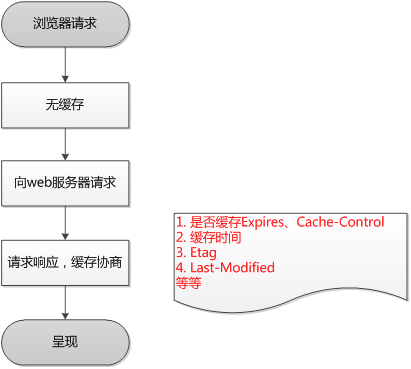
\includegraphics[width=0.8\textwidth]{./images/firstRequest.png}  
\end{figure}

下一次请求

\begin{figure}[!ht]
    \centering    
     \caption{\label{Fig:async} Asynchronous I/O model}
    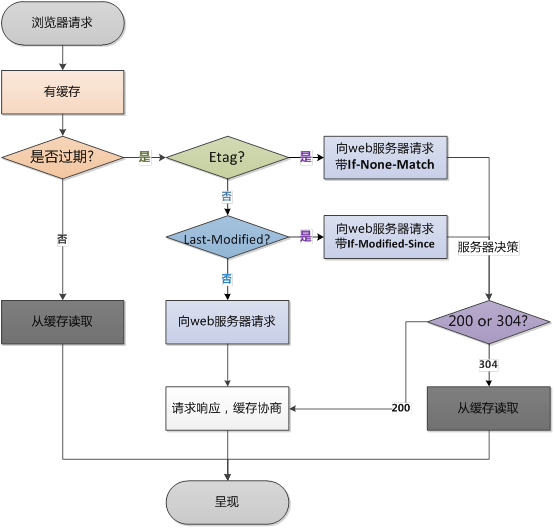
\includegraphics[width=0.8\textwidth]{./images/nextRequest.png}  
\end{figure}

\subsection{强缓存}

运维了解到此基础就OK, 需要了解更深可以查看网上资源

https://www.zhihu.com/question/20790576

https://www.cnblogs.com/wonyun/p/5524617.html

\section{linux系统命令}

用户权限分配

用户/组   主机    可以切换的用户角色	命令
root     ALL=     (ALL)			ALL
User_Alias  Host_Alias    Runas_Aliase  Cmad_Alias  
mikem
%groupname



\begin{thebibliography}{9}
\bibitem{latexcompanion} 
Michel Goossens, Frank Mittelbach, and Alexander Samarin. 
\textit{The \LaTeX\ Companion}. 
Addison-Wesley, Reading, Massachusetts, 1993.
 
\bibitem{einstein} 
Albert Einstein. 
\textit{Zur Elektrodynamik bewegter K{\"o}rper}. (German) 
[\textit{On the electrodynamics of moving bodies}]. 
Annalen der Physik, 322(10):891–921, 1905.
 
\bibitem{knuthwebsite} 
Knuth: Computers and Typesetting,
\\\texttt{http://www-cs-faculty.stanford.edu/\~{}uno/abcde.html}

\bibitem{execredirect}
	丘迟: exec重定向以及io重定向
	\\\texttt{http://xstarcd.github.io/wiki/shell/exec_redirect.html}

\end{thebibliography}


\end{document}
